\documentclass[12pt]{article}
\usepackage{amsmath,amsthm,amssymb,fullpage,graphicx}

\newtheorem{thm}{Theorem}[section]
\newtheorem{lemma}[thm]{Lemma}
\newtheorem{prop}[thm]{Proposition}
\newtheorem{cor}[thm]{Corollary}
\newtheorem{rem}[thm]{Remark}
\newtheorem{defn}[thm]{Definition}

     \def\NN{\mathbb{N} }
     \def\ZZ{\mathbb{Z} }
     \def\QQ{\mathbb{Q} }
     \def\RR{\mathbb{R} }
     \def\CC{\mathbb{C} }
     \def\f{\frac }
     \def\b{\begin }
     \def\e{\end }


\setcounter{page}{8}
\b{document}

\setcounter{section}{3}


\section{Numerical Simulations of Rogue Waves Solutions}


\begin{figure}[h]
\begin{center}
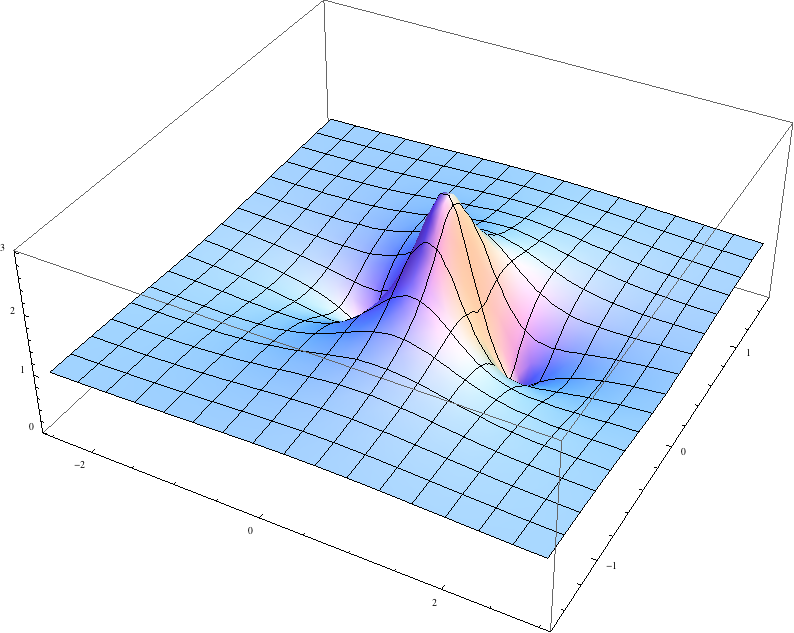
\includegraphics[width=250px]{1st_order.png}\\
Figure 1: Mathematica plot of 1st order rogue wave solution.
\end{center}
\end{figure}
\vspace{-1mm}

\begin{figure}[h]
\begin{center}
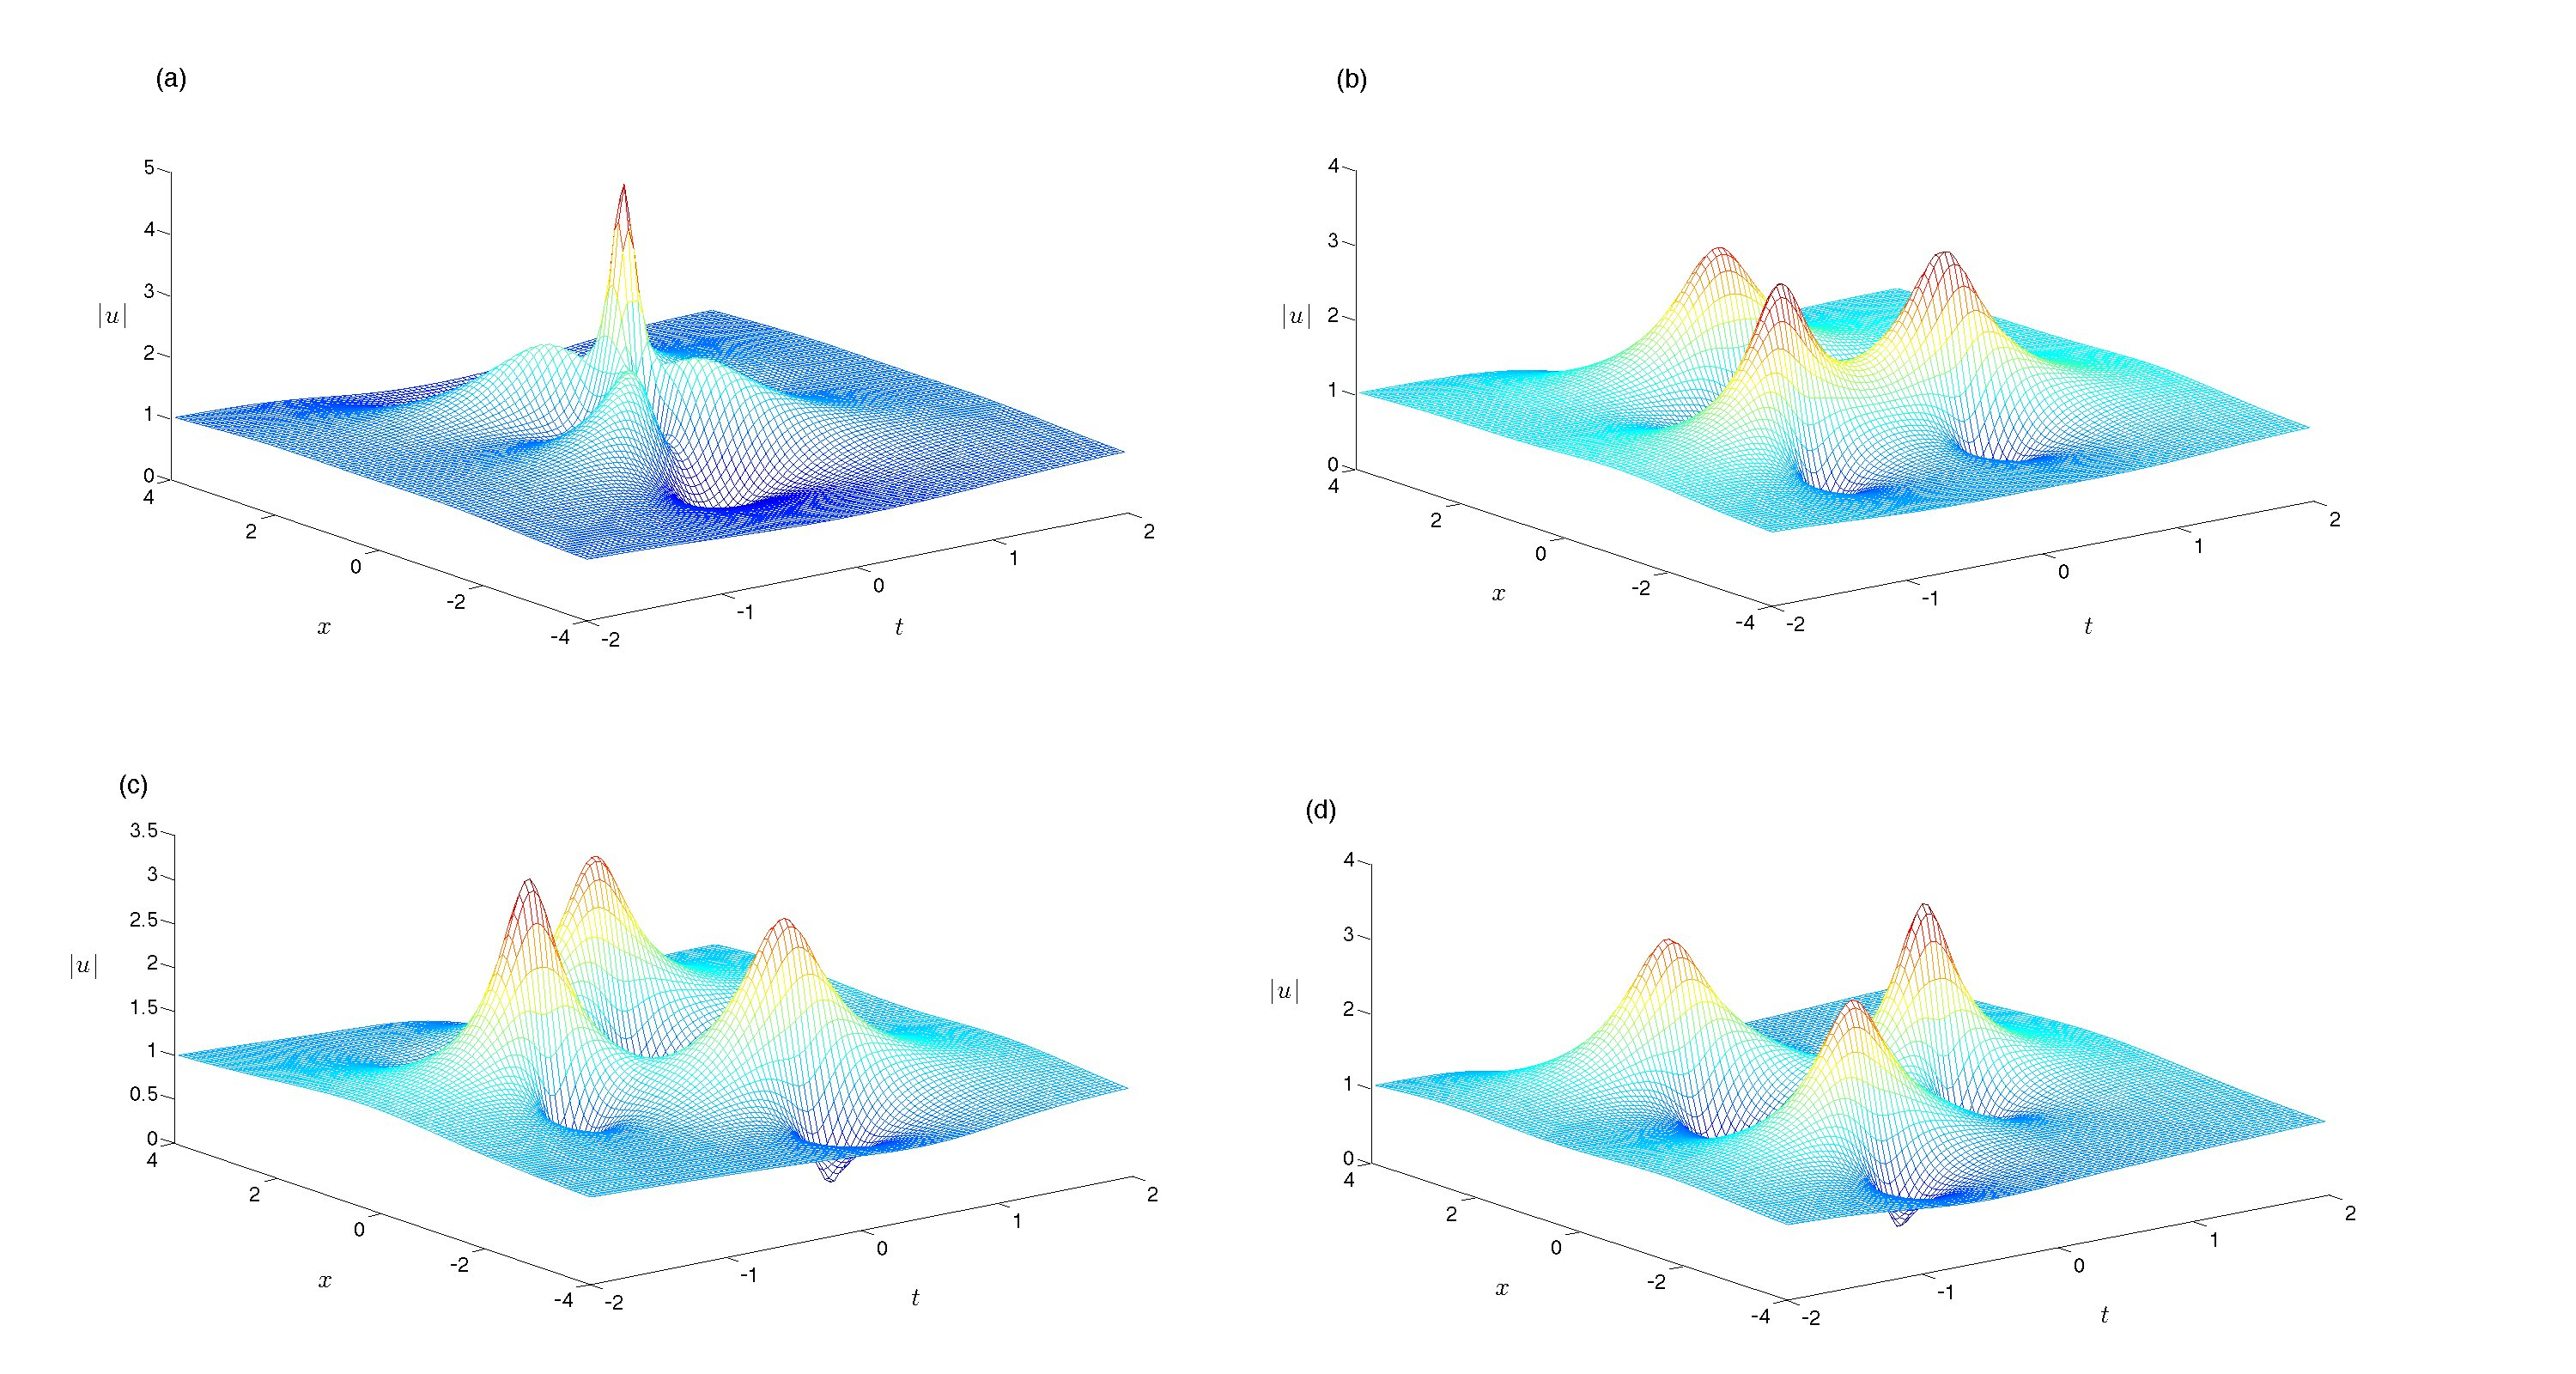
\includegraphics[width=330px]{figure1_new.jpg}\\
Figure 2: 2nd order wave solutions plotted in MATLAB for the following values of $a_3$:\\
(a) -1/12, (b) 5/3, (c) $-5i/2$, and (d) $5i/2$.
\end{center}
\end{figure}
\vspace{-1mm}

\begin{figure}
\begin{center}
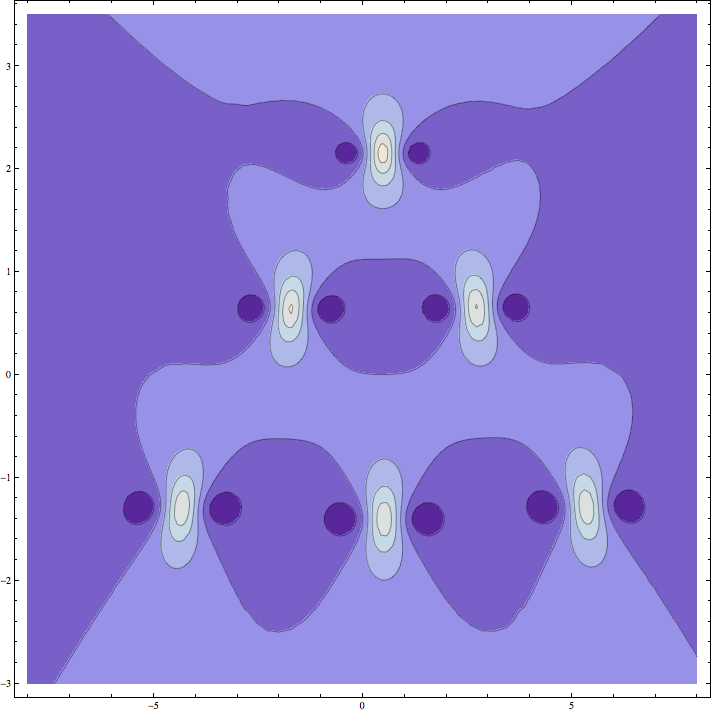
\includegraphics[width=275px]{3rd_order_many_peaks_contour.png}\\
Figure 3: Mathematica contour plot of 3rd order solution for $(a_3,a_5)=(25i/3,0)$ showing 6 intensity humps.
\end{center}
\end{figure}
\vspace{-1mm}

\begin{figure}
\begin{center}
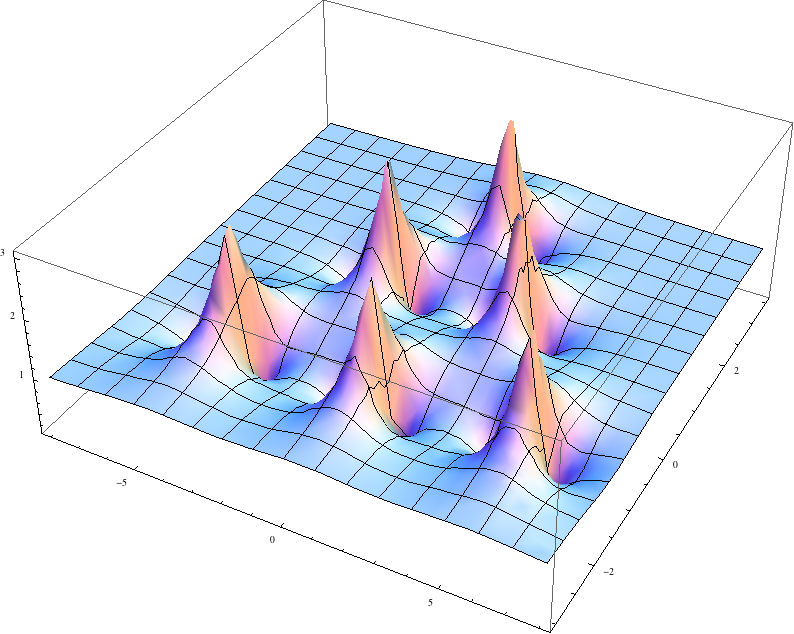
\includegraphics[width=300px]{3rd_order_many_peaks.png}\\
Figure 4: Mathematica plot of 3rd order solution for $(a_3,a_5)=(25i/3,0)$.
\end{center}
\end{figure}
\vspace{-1mm}

\begin{figure}
\begin{center}
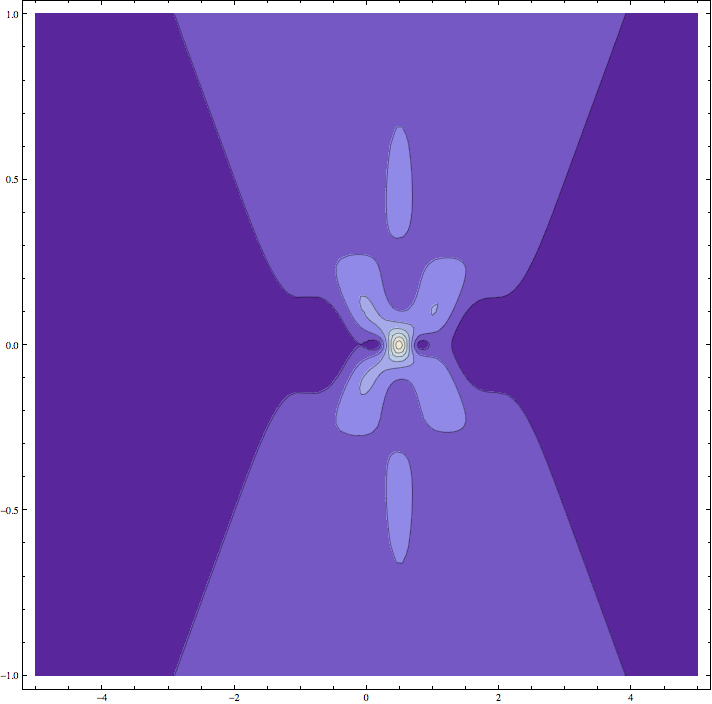
\includegraphics[width=300px]{3rd_order_max_peak_contour.png}\\
Figure 5: Mathematica contour plot of 3rd order solution for $(a_3,a_5)=(-1/12,-1/240)$ which achieves a maximum amplitude of 9 at $(x,t)=(1/2,0)$.
\end{center}
\end{figure}
\vspace{-1mm}

\begin{figure}
\begin{center}
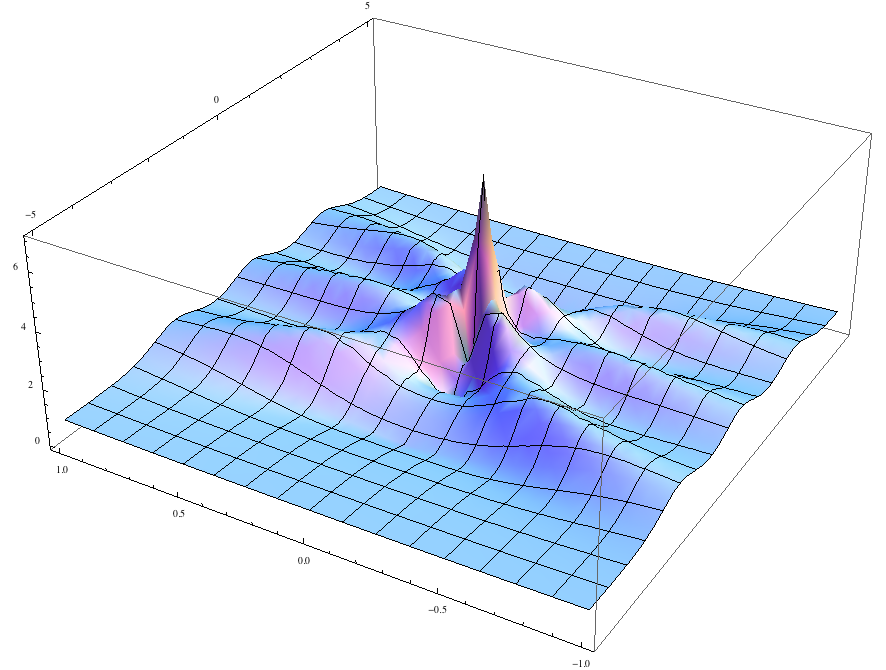
\includegraphics[width=300px]{3rd_order_max_peak.png}\\
Figure 6:  Mathematica plot of 3rd order solution for $(a_3,a_5)=(-1/12,-1/240)$.
\end{center}
\end{figure}
\vspace{-1mm}

\begin{figure}
\begin{center}
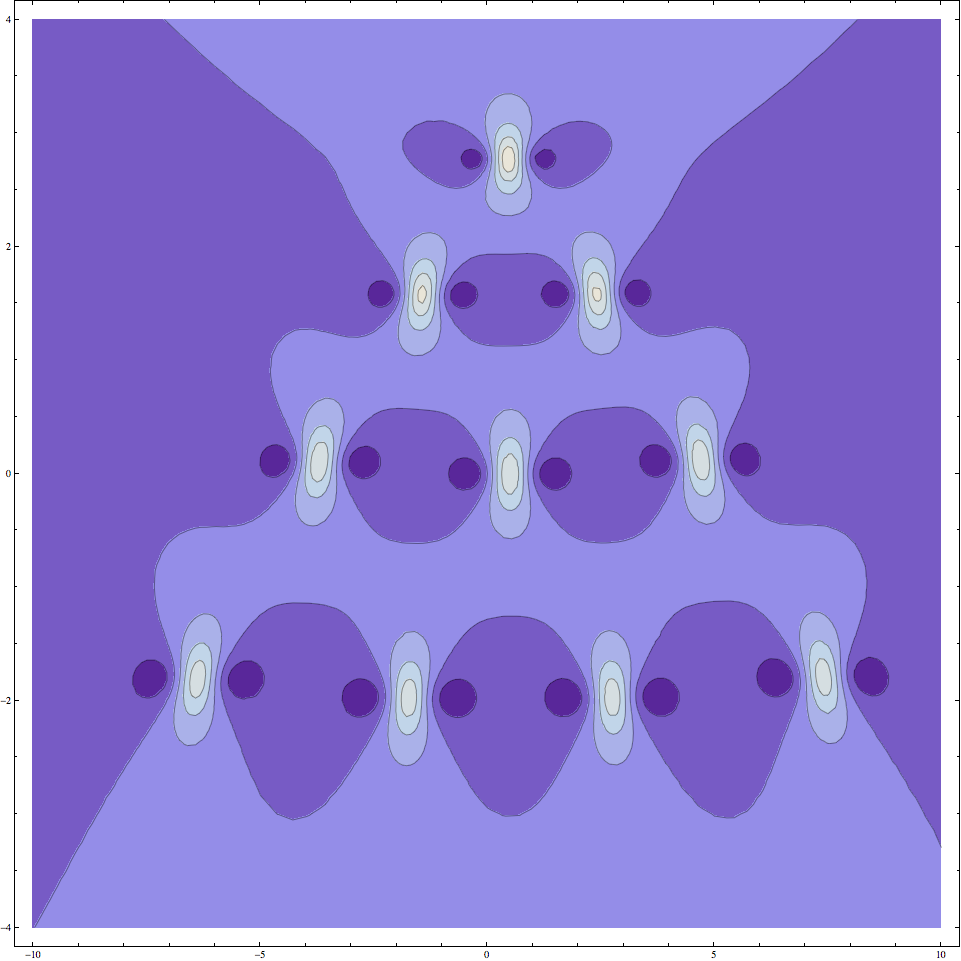
\includegraphics[width=300px]{4th_order_many_peaks_contour.png}\\
Figure 7: Mathematica contour plot of 4rd order solution for $(a_3,a_5,a_7)=(25i/3,0,0)$ showing 10 intensity humps.
\end{center}
\end{figure}
\vspace{-1mm}

\begin{figure}
\begin{center}
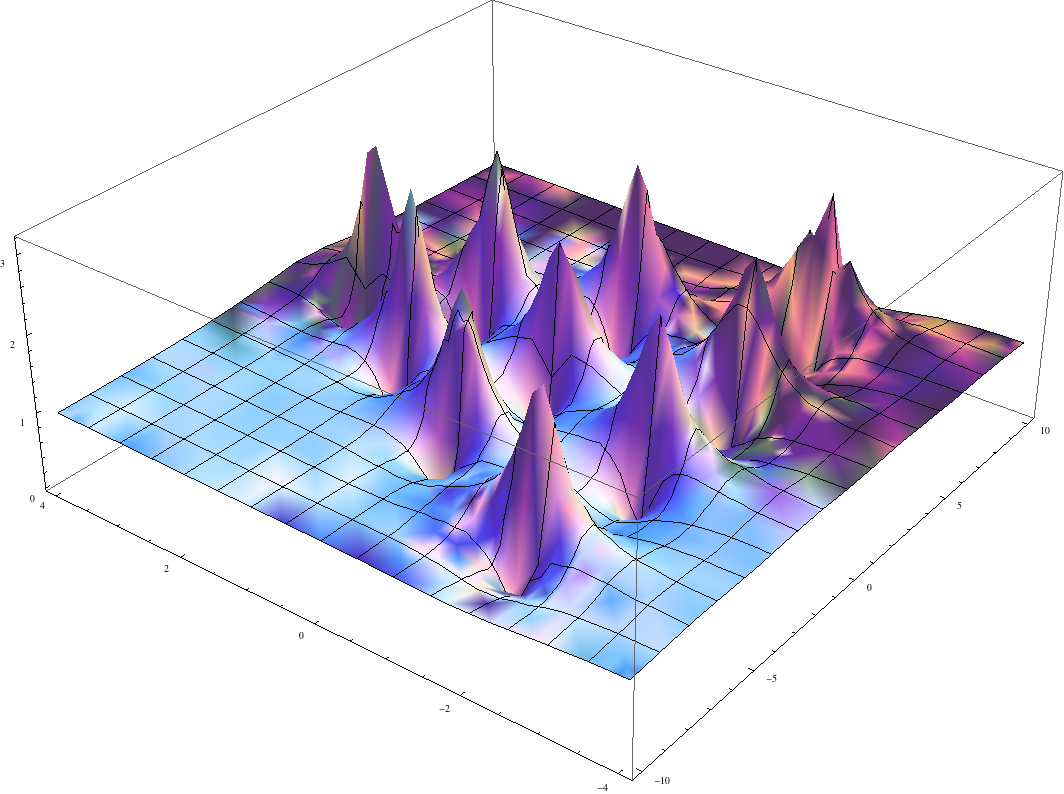
\includegraphics[width=300px]{4th_order_many_peaks.png}\\
Figure 8: Mathematica plot of 4rd order solution for $(a_3,a_5,a_7)=(25i/3,0,0)$.
\end{center}
\end{figure}
\vspace{-1mm}

\begin{figure}
\begin{center}
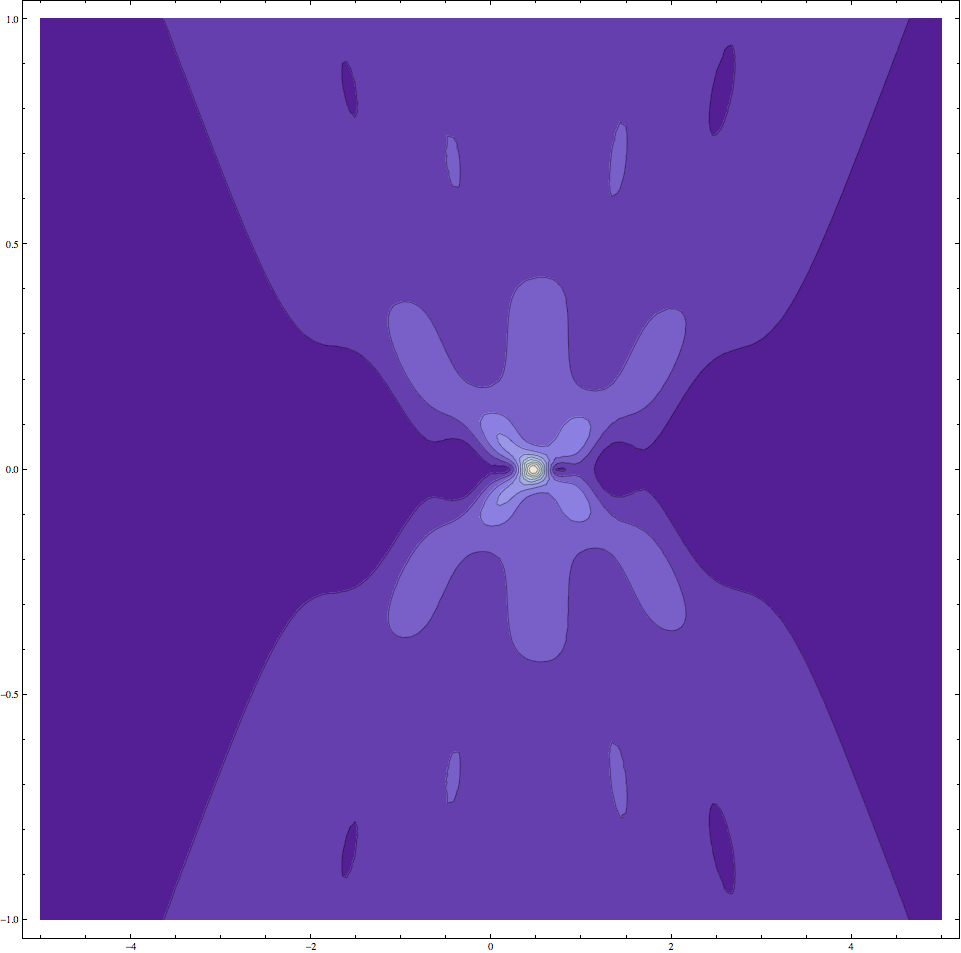
\includegraphics[width=300px]{4th_order_max_peak_contour.png}\\
Figure 9: Mathematica contour plot of 4rd order solution for $(a_3,a_5,a_7)=(-1/12,-1/240,0)$, which achieves a maximum amplitudeof 9 also at $(1/2,0)$. 
\end{center}
\end{figure}
\vspace{-1mm}

\begin{figure}
\begin{center}
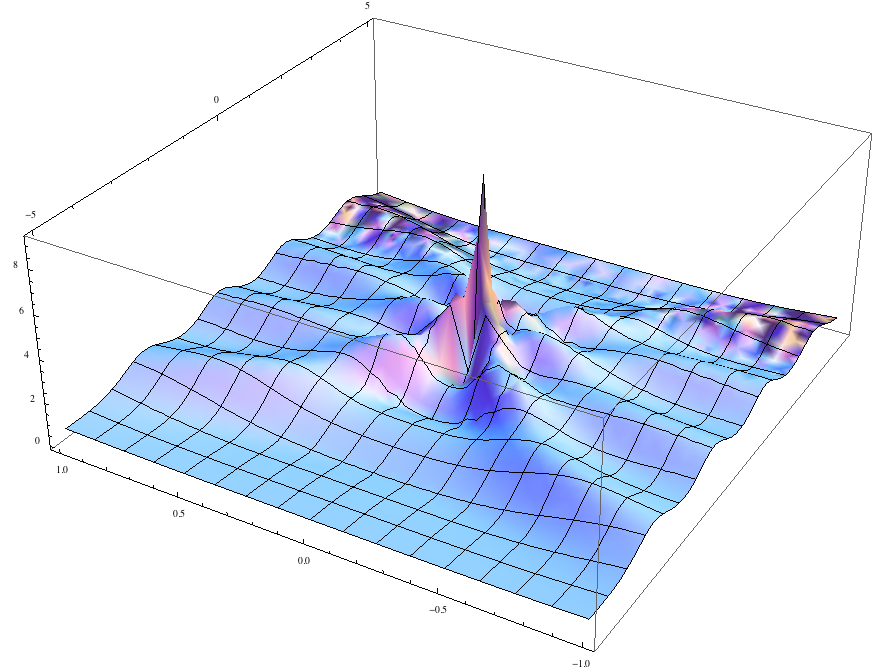
\includegraphics[width=300px]{4th_order_max_peak.png}\\
Figure 10: Mathematica plot of 4rd order solution for $(a_3,a_5,a_7)=(-1/12,-1/240,0)$.
\end{center}
\end{figure}
\vspace{-1mm}

\begin{figure}
\begin{center}
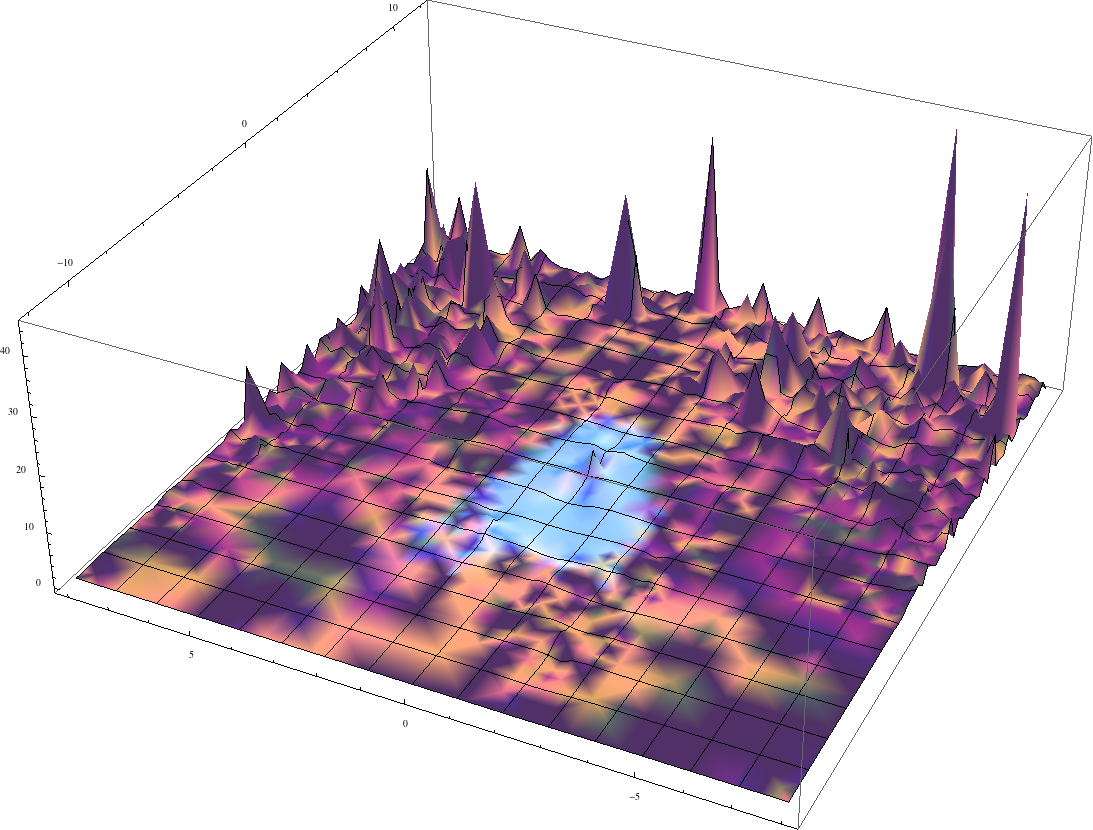
\includegraphics[width=450px]{5th_order_unstable.png}\\
Figure 11: Mathematica plot of 5th order solution for $(a_3,a_5,a_7,a_9)=(-1/12,-1/240,0,0)$ showing the extreme instability of such high order solutions. At $(x,t)=(1/2,0)$ this achieves a maximum amplitude of 11.
\end{center}
\end{figure}
\vspace{-1mm}


\e{document}